\section{Problemi Insolubili e Riducibilità}

In questo capitolo studieremo i problemi di appartenenza o di non appartenenza di un elemento ad un dato insieme, affrontando così il modo di risolvere problemi alternativo a quello considerato fino ad ora, in cui l'oggetto del discorso era calcolare funzioni.\
Ovviamente queste due visioni di un problema matematico sono strettamente correlate; in seguito vedremo \textit{esattamente} come lo sono.

Ricordiamo la definizione di insieme ricorsivo.

\vspace{12pt}
\noindent Un insieme $I$ è \textit{ricorsivo} (ovvero \textit{decidibile}) se e solo se la sua funzione caratteristica
\[\chi_I(x)=\left\{\begin{array}{l l}
        1 & \text{se } x\in I       \\
        0 & \text{se } x \not \in I \\
    \end{array}\right.\]
è calcolabile totale.\

Vediamo quali insiemi vengono fuori se non poniamo alcun limite al numero dei passi consentiti a una macchina.\
Significa che andremo a vedere se una MdT termina (su un particolare dato) e se c'è un algoritmo per determinare tale proprietà -- ovviamente no!\
Il gioco si fa definendo una classe di insiemi più ampia di quella degli insiemi ricorsivi.

\begin{definition}
    \label{rec_enumerabile}
    Diciamo che un insieme $I$ è \textit{ricorsivamente enumerabile}
    \[I\ \mathrm{\grave{e}}\ \mathit{ricorsivamente\ enumerabile\ sse}\  \exists i.\ I = dom(\varphi_i)\]
\end{definition}

\noindent Un insieme ricorsivamente enumerabile, detto anche \textit{semi-decidibile} è quindi il dominio di una funzione calcolabile (il più delle volte \textit{parziale}, infatti se fosse totale $I = \mathbb{N}$), che è anche detta \textit{semi-caratteristica} di $I$.\

Ci sono ovvie relazioni tra gli insiemi ricorsivi (decidibili) e quelli ricorsivamente enumerabili (semi-decidibili).\

\begin{property}
    \label{R-RE}
    \hfill
    \begin{itemize}
        \item [i)] Se $I$ è ricorsivo allora $I$ è ricorsivamente enumerabile.
        \item [ii)] $I, \bar{I}$ sono ricorsivamente enumerabili se e solo se $I$ (e $\bar{I}$) sono ricorsivi.
    \end{itemize}
\end{property}

\begin{proof}
    Il caso (i) è ovvio:\ la $\varphi_i$ cercata restituisce 1 su $x$ se $\chi_I(x)=1$, altrimenti diverge.\

    (ii) Il caso precedente basta per vedere la parte ``\textit{se}''.\
    Consideriamo allora la parte ``\textit{solo se}'':\ siano $\varphi_i$ e $\varphi_{\bar{i}}$ le funzioni i cui domini sono rispettivamente $I$ e $\bar{I}$.\
    Adesso si ripeta il seguente ciclo:\ esegui un passo nel calcolo di $\varphi_i(x)$; se $\varphi_i(x) \downarrow$ allora $x \in I$ e poni $\chi_I(x) = 1$; altrimenti esegui un passo nel calcolo di $\varphi_{\bar{i}}(x)$; se $\varphi_{\bar{i}}(x) \downarrow$ allora $x \notin I$ e poni $\chi_I(x)=0$.\
\end{proof}

\noindent In realtà uno vorrebbe poter elencare (enumerare, generare) gli elementi di un insieme mediante una funzione calcolabile.\
Ecco un teorema che ci permette di fare ciò.\

\begin{theorem}
    $I$ è ricorsivamente enumerabile se e solamente se è vuoto oppure è l'immagine di una funzione calcolabile totale.\
\end{theorem}

\begin{proof}
    Il primo caso si dimostra banalmente:\ l'insieme vuoto è il dominio di una funzione ovunque indefinita; d'altra parte, la funzione ovunque indefinita ha dominio vuoto.\

    Consideriamo adesso il caso in cui $I = dom(\varphi_i)$ sia non vuoto:\ consiste nella costruzione di una funzione totale calcolabile $f$ tale che $I=imm(f)$ a partire da $\varphi_i$.\
    Innanzitutto, si cerca un elemento di $I$ mediante un procedimento a coda di colomba (Figura \ref{fig:coda di colomba}), in cui l'indice di riga $m$ rappresenta il numero dei passi del calcolo di $\varphi_i$ e l'indice di colonna $n$ il suo argomento.\
    \begin{figure}[H]
        \centering
        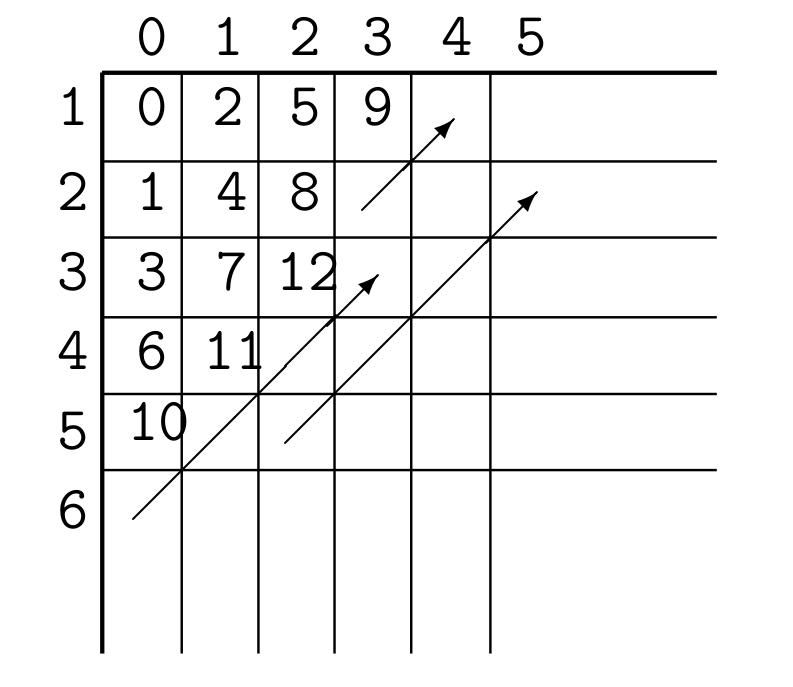
\includegraphics[width=0.4\textwidth]{codadicolomba_da1}
        \caption{Nella tabella a ``coda di colomba'' si interpreti l'indice di riga come il numero di passi eseguiti da $M_i$ sul valore dell'indice di colonna.}
        \label{fig:coda di colomba}
    \end{figure}

    \noindent Più precisamente, si eseguono $m$ passi nel calcolo di $\varphi_i(n)$, finché per qualche valore di $m$ e dell'argomento, sia $\bar{n}$, il calcolo si arresta; ovvero $\varphi_i(\bar{n})\downarrow$ in $m$ passi e quindi $\bar{n} \in I$.\

    A questo punto, rappresentando con $\langle n,m\rangle$ il valore della codifica della coppia $(n,m)$, si inizia un secondo procedimento a coda di colomba eseguendo $\varphi_i(n)$ per $m$ passi:\ se tale calcolo si arresta, allora si pone $f(\langle n,m\rangle) = n$ (ovviamente $n \in dom(\varphi_i)= I$), altrimenti si pone $f(\langle n,m\rangle) = \bar{n}$ (per quanto detto prima $\bar{n} \in I$); si itera il procedimento incrementando la codifica $\langle n,m\rangle$, ovvero considerando $\langle n, m\rangle + 1$.\
    Si generano così tutti gli elementi di $I$.\

\end{proof}

\noindent Adesso vediamo un insieme veramente speciale e paradigmatico:
\[K = \{ x \mid \varphi_x(x) \downarrow\}\]

\begin{property}
    \label{RE}
    $K$ è ricorsivamente enumerabile.
\end{property}

\begin{proof}
    $K$ è il dominio di
    \[\psi(x) = \left\{\begin{array}{l l}
            x                   & \mathrm{se}\ \varphi_x(x)\downarrow \\
            \mathrm{indefinita} & \mathrm{altrimenti}                 \\
        \end{array}\right.\]
    che è calcolabile:\ prendi la MdT $M_x$ e applicala a $x$; se e quando essa si arresta, restituisci $x$.
\end{proof}

\noindent Facciamo adesso vedere che la $\psi$ della dimostrazione precedente genera $K$, ma \textit{non} è una funzione calcolabile totale, e che nessuna funzione che decida $K$ lo è.\

\begin{property}
    \label{K_notRec}
    $K$ non è ricorsivo.\
\end{property}

\begin{proof}
    Sia $\chi_K$ la funzione caratteristica di $K$ e per assurdo sia totale e calcolabile.\
    Ma allora anche la seguente funzione
    \[f(x)=\left\{\begin{array}{l l}
            \varphi_x(x) + 1 & \mathrm{se}\ x \in K    \\
            0                & \mathrm{se}\ x \notin K \\
        \end{array}\right.\]
    sarebbe calcolabile totale.\
    In questo modo otteniamo una contraddizione perché $\forall x.\ f(x) \neq \varphi_x(x)$; quindi non troviamo alcun indice per $f$ che di conseguenza non è calcolabile.\
\end{proof}

\noindent La proprietà appena vista significa che \textit{non esiste un algoritmo per decidere se} $x \in K$ o no.\
Quindi questo problema è \textit{insolubile}, anche se ovviamente è semi-decidibile.\
Inoltre $\overline{K}$ \textit{non è ricorsivamente enumerabile} quindi esistono problemi ancora più difficili di $K$!\
Infatti, se $\overline{K}$ fosse ricorsivamente enumerabile, sia $K$ che $\overline{K}$ sarebbero ricorsivi, per la proprietà \ref{R-RE}(ii), in quanto $K$ è ricorsivamente enumerabile per la proprietà \ref{RE}.\
Abbiamo così stabilito un piccolo frammento di gerarchia:
\[R\subsetneq RE \subsetneq \mathit{non}RE\]
dove $R$ è la classe degli insiemi ricorsivi, $RE$ quella degli insiemi ricorsivamente enumerabili e $\mathit{non}RE$ quella degli insiemi non ricorsivamente enumerabili (la scelta del nome ``non ricorsivamente enumerabile'' non è molto felice, perché un insieme (ricorsivo è anche) ricorsivamente enumerabile è anche non ricorsivamente enumerabile:\ in questo, come in mille altri casi, una formula è assai più precisa di una frase nel linguaggio comune!\ con maggior esattezza si dovrebbe dire che $\overline{K} \in \mathit{co\textrm{-}}RE$, la classe dei problemi i cui complementi sono ricorsivamente enumerabili, ma non ricorsivi).

\vspace{12pt}

\noindent Finalmente siamo arrivati al problema, che di solito si chiama \textit{problema della fermata}, e che confuta l'affermazione di Hilbert che \textit{tutti} i problemi matematici hanno una caratterizzazione esatta.\
A costo di essere noioso, vale la pena di ripetere che, come tutti i risultati sulla calcolabilità che discuteremo, anche questo è \textit{indipendente} sia dal formalismo impiegato per scrivere gli algoritmi, ovvero per esprimere le funzioni, sia dall'enumerazione effettiva scelta.\
In altre parole, \textit{tutti} i formalismi che siano T-equivalenti soffrono del problema della fermata, il che potrebbe, con le dovute ipotesi, essere aggiunto come terzo punto al teorema di espressività.\

Potrebbe comunque rimanere il dubbio che $K$ sia un problema artificiale, che non ha alcuna rilevanza pratica; si tratterebbe allora di un risultato negativo, ma di scarso impatto sulla realizzazione di elaboratori, programmi e degli altri aggeggi infernatici che ci stanno a cuore.\
Infatti a chi mai verrebbe in mente di applicare un programma a sé stesso?\
A chi realizza compilatori, in particolare il cosiddetto ``bootstrapping''!\
Il problema può essere raccontato così:\ supponete di aver scritto un compilatore, o meglio un \textit{cross-compiler}, in un certo linguaggio $L$, che traduce programmi scritti in $L$ in programmi scritti in un altro linguaggio $A$; rappresentiamo tale compilatore come $C_L^{L \rightarrow A}$ --- questo ovviamente implica che abbiate già un compilatore per $L$ che gira su una qualche macchina, magari molto potente, ma sulla quale i programmi $A$ non girano.\
Supponete adesso di voler scrivere il compilatore $C_A^{L\rightarrow A}$, cioè un compilatore ancora da $L$ a $A$, ma stavolta scritto nel liguaggio $A$, che potrebbe essere l'assembler di una macchina che non sostiene $L$.\
Basta allora prendere $C_L^{L\rightarrow A}$, applicarlo a sé stesso per ottenere ciò che si desidera:
\[C_L^{L\rightarrow A} (C_L^L\rightarrow A) = C_A^{L\rightarrow A}\]
Tuttavia questo può ancora sembrare un caso estremo, e consideriamo allora il seguente problema, la cui soluzione positiva ci aiuterebbe enormemente nel nostro lavoro.\
Possiamo scrivere un programma $P$ che, dato un altro programma $Q$ (individuato dal suo indice $y$) e un argomento $x$, ci assicura che la computazione di $Q$ su $x$ terminerà o meno?\
Questo è un problema certamente più reale di  $K$, prescinde dalla formalizzazione di algoritmo che stiamo esaminando e ha dunque interesse in sé.\
Infatti, piacerebbe a ciascuno di noi avere a disposizione il programma guardia $P$, in modo da non lanciare nemmeno l'esecuzione di $Q(x)$ quando questi non termina.\
Vista la sua importanza, questo problema si merita un nome:\

\begin{table}[H]
    \centering
    \begin{tabular}{|l|}
        \hline
        \textbf{Problema della fermata}:\ dati $x,y.\ \varphi_y(x)\downarrow$?\ cioè $P_y(x)$ si ferma? \\\hline
    \end{tabular}
\end{table}

\noindent Il problema della fermata si formalizza e si studia nei termini usati in questo capitolo introducendo un altro insieme che gode di grande popolarità e caratterizzandone la natura.\
Sia
\[K_0 = \{(x,y) \mid \varphi_y(x)\downarrow\},\ \mathrm{ovvero}\ K_0 = \{(x,y) \mid \exists z.\ T(x,y,z)\} \]
dove $T$ è il predicato di Kleene che abbiamo introdotto nel teorema di forma normale (\ref{forma normale}).

\begin{corollario}
    $K_0$ non è ricorsivo.
\end{corollario}

\begin{proof}
    Si ha che $x \in K$ se e solamente se $(x,x) \in K_0$, quindi se $K_0$ fosse ricorsivo lo sarebbe anche $K$.
\end{proof}

\noindent Abbiamo appena visto che il problema della fermata, formalizzato da $K_0$, è strettamente collegato al problema per decidere l'appartenenza o meno di un elemento a $K$, tanto da risultarne ``equivalente''.\
La tecnica di dimostrazione usata per collegare $K$ e $K_0$ si basa sul concetto di {\footnotesize RIDUCIBILITÀ}, che è una nozione fondamentale, e non solo nella teoria della calcolabilità e della complessità.\
Il punto cruciale nella sua definizione è che la \textit{funzione di riduzione} deve essere ``\textit{semplice}'' (in questa parte del corso useremo funzioni calcolabili totali, nella terza parte funzioni polinomiali in tempo o indifferentemente logaritmiche in spazio).\

Visto che la nozione di riducibilità è importantissima, faremo di seguito una digressione per introdurla e caratterizzarla in una forma abbastanza generale.

\vspace{24pt}
\noindent\hrulefill

\noindent\hrulefill RIDUCIBILITÀ\hrulefill

\vspace{6pt}
\noindent Una riduzione è una particolare funzione $f$ che trasforma un problema (ovvero un insieme o una classe) $A$ in un altro problema $B$, in modo da mantenerne inalterata la caratteristica principale.

\begin{definition}
    \label{riduzione}
    $A$ si \textit{riduce} a $B$ secondo la \textit{riduzione} $f$, in simboli $A \leqslant_f B$, tutte e sole le volte che
    \[a \in A \Leftrightarrow f(a) \in B,\ \mathrm{ovvero}\ f(A) \subseteq B\ \mathrm{e}\ f(\bar{A}) \subseteq \overline{B}\]
\end{definition}

\noindent La seguente proprietà è di immediata dimostrazione.

\begin{property}
    \label{riduzione_prop}
    $A \leqslant_f B$ se e solamente se $\bar{A} \leqslant_f \overline{B}$.
\end{property}

\begin{proof}
    Si ha che $x \in \bar{A}$ se e solamente se $x \notin A$ se e solamente se $f(x) \notin B$ se e solamente se $f(x) \in \overline{B}$.
\end{proof}

\noindent Più in generale, si definisce una relazione di riduzioni ($\leqslant_F$) dove $F$ è una particolare classe di funzioni.\
Allora scriveremo
\[A \leqslant_F B \Leftrightarrow \exists f \in F.\ A\leqslant_f B\]
Ci interessano solo quelle riduzioni $\leqslant_F$ che danno origine a \textit{classi} di problemi in qualche modo ``omogenei''.\
Vediamo adesso in maggior dettaglio cosa si debba intendere per omogeneo e come si possano definire quelle relazioni di riduzione che riteniamo interessanti.\

\begin{definition}
    \label{classificazione}
    Siano $\mathcal{D}$ e $\mathcal{E}$ due classi di problemi con $\mathcal{D} \subseteq \mathcal{E}$ (e anche $\mathcal{E} \subseteq \mathcal{H}$, che però non menzioneremo ulteriormente).\
    Una relazione di riduzione $\leqslant_F$ \textit{classifica} $\mathcal{D}$ ed $\mathcal{E}$ se e solo se per ogni problema $A,B,C$

    \begin{itemize}
        \item[i)] $A \leqslant_F A$ \hfill (\textit{\footnotesize Riflessiva})
        \item[ii)] $A \leqslant_F B, B \leqslant_F C$ implica $A \leqslant_F C$ \hfill (\textit{\footnotesize Transitiva})
        \item[iii)] $A \leqslant_F B, B \in \mathcal{D}$ implica $A \in \mathcal{D}$ \hfill (\textit{\footnotesize $\mathcal{D}$ ideale = chiuso all'ingiù per riduzione})
        \item[iv)] $A \leqslant_F B, B \in \mathcal{E}$ implica $A \in \mathcal{E}$ \hfill (\textit{\footnotesize $\mathcal{E}$ ideale = chiuso all'ingiù per riduzione})
    \end{itemize}
\end{definition}

\noindent Vediamo adesso una caratterizzazione differente, ma del tutto equivalente, delle riduzioni che classificano coppie di classi, l'una inclusa nell'altra.

\begin{lemma}
    \label{classificazione_lemma}
    Una relazione di riduzione $\leqslant_F$ classifica $\mathcal{D}$ ed $\mathcal{E}$, tali che $\mathcal{D} \subseteq \mathcal{E}$, se e solo se
    \begin{itemize}
        \item[i)] $\mathit{id} \in F$ \hfill ($F$ ha identità)
        \item[ii)] $f,g \in F \Rightarrow f \circ g \in F$ \hfill ($F$ chiusa per composizione)
        \item[iii)] $f \in F,\ B \in \mathcal{D} \Rightarrow \{x \mid f(x) \in B\} \in \mathcal{D}$
        \item[iv)] $f \in F,\ B \in \mathcal{E} \Rightarrow \{x \mid f(x) \in B\} \in \mathcal{E}$
    \end{itemize}
\end{lemma}

\begin{proof}
    Vedi punto per punto la definizione di classificazione.
\end{proof}

\noindent Attraverso il concetto di relazione di riduzione che classifica due classi di problemi si possono definire le seguenti nozioni molto importanti.\
(Si noti che la relazione $\leqslant_F$ è un pre-ordine parziale\footnote{Cioè un ordinamento parziale riflessivo e transitivo, ma non anti-simmetrico.}, il che giustifica l'uso del termine ``ideale'' fatto sopra.)

\newpage

\begin{definition}
    \label{arduo_completo}
    Se $\leqslant_F$ classifica $\mathcal{D}$ ed $\mathcal{E}$, $\forall A,B,H$ problemi
    \begin{itemize}
        \item[i)] $A\equiv B$ se $A \leqslant_F B$ e $B \leqslant_F A$ (si dice anche che $\{B \mid A \equiv_F B\}$ è il \textit{grado} di $A$, o anche che $A$ è equivalente a $B$ rispetto a $\leqslant_F$)\footnote{Se consideriamo, per esempio $\mathcal{D}_{\equiv}$ allora $\leqslant_F$ diventa un ordinamento parziale.}.
        \item[ii)] $H$ è $\leqslant_F$-\textit{arduo} per $\mathcal{E}$ se $\forall A \in \mathcal{E}.\ A \leqslant_F H$ \footnote{Potrebbe essere $H \in \mathcal{H}\backslash\mathcal{E}$.}.
        \item[iii)] $H$ è $\leqslant_F$-\textit{completo} per $\mathcal{E}$ se $H$ è $\leqslant_F$-arduo per $\mathcal{E}$ e $H \in \mathcal{E}$.
    \end{itemize}
    Diremo semplicemente $\mathcal{E}$-arduo o $\mathcal{E}$-completo quando la classe di riduzioni $F$ è fissata; talvolta ometteremo anche $\mathcal{E}$, se chiaro nel contesto.

\end{definition}

\begin{figure}[H]
    \centering
    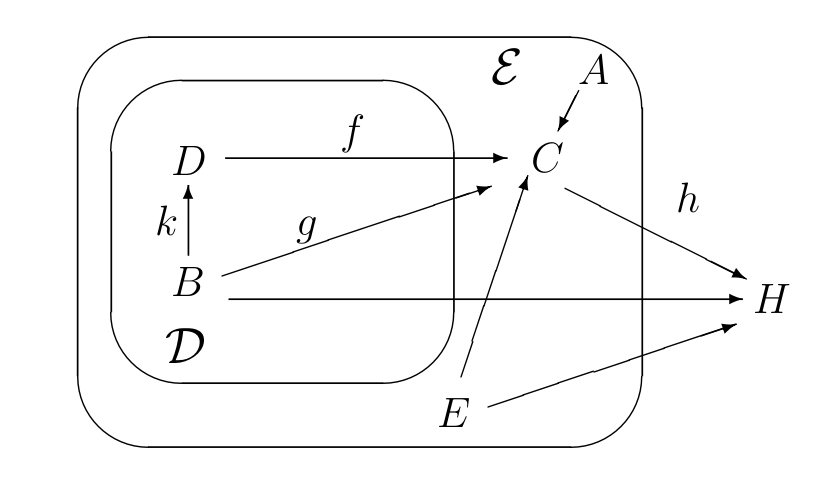
\includegraphics[width=0.6\textwidth]{riducibilita}
\end{figure}

\noindent Il disegno di sopra esemplifica quanto scritto.\
Il problema $C$ è completo per $\mathcal{E}$ e a esso si riducono sia $B$ e $D$ di $\mathcal{D}$, sia $A$ e $E$ di $\mathcal{E}$; non tutte le riduzioni sono state disegnate (come frecce), tuttavia si noti che $g = f \circ k$ e allo stesso modo si compongono tutte le frecce disegnate o meno; infine $H$ è un problema arduo per $\mathcal{E}$, ma non completo:\ tutti i problemi di $\mathcal{E}$ si riducono ad $H$, ma $H \notin \mathcal{E}$.

Se un problema è completo per un classe $\mathcal{E}$ e appartiene ad un sottoclasse $\mathcal{D}$, allora le due classi coincidono.\

\begin{property}
    Se $\leqslant_F$ classifica $\mathcal{D}$ ed $\mathcal{E}$, $\mathcal{D} \subseteq \mathcal{E}$ e $C$ è completo per $\mathcal{E}$, allora $C \in \mathcal{D}$ se e solamente se $\mathcal{D} = \mathcal{E}$.\
\end{property}

\begin{proof}
    (se) ovvia.\

    \noindent(solo se) Sia $C \in \mathcal{D}$ e $A \in \mathcal{E}$.\
    Per completezza $A \leqslant_F C$ e $A \in \mathcal{D}$ per la condizione (iii) di $\leqslant_F$ che classifica $\mathcal{D}$ ed $\mathcal{E}$.\
    Quindi $\mathcal{E} \subseteq \mathcal{D}$ e la tesi.
\end{proof}

\noindent Inoltre è facile capire quali siano gli elementi del grado di $A$, problema $\leqslant_F$-completo per $\mathcal{E}$.\
Per aiutare l'intuizione guardiamo nuovamente il disegno fatto sopra:\ se vi fosse una riduzione anche tra $C$ e $A$, allora componendo le frecce si otterrebbe una riduzione tra ogni elemento di $\mathcal{E}$ e $A$, cioè anche $A$ sarebbe completo per $\mathcal{E}$.

\begin{property}
    Se $A$ è completo per $\mathcal{E}$, $A \leqslant_F B$ e $B \in \mathcal{E}$, allora $B$ è completo per $\mathcal{E}$.
\end{property}

\begin{proof}
    $\forall D \in \mathcal{E}$, $D \leqslant_F A$ per complettezza, ma $\leqslant_F$-classifica $\mathcal{D}$ ed $\mathcal{E}$ e allora $D \leqslant_F A$ e $A \leqslant_F B$ implicano $D \leqslant_F B$ e quindi $B$ è arduo e, poiché appartiene a $\mathcal{E}$, è completo.
\end{proof}

\noindent Un problema completo per $\mathcal{E}$ gioca un ruolo rilevantissimo, in quanto ``rappresenta la difficoltà'' massima dei problemi di $\mathcal{E}$.\
Infatti, è facile vedere che il grado di un problema $A$ completo per $\mathcal{E}$ è il grado massimo di $\mathcal{E}$ in $\leqslant_F$.\
Inoltre, valgono le seguenti affermazioni (anche per problemi non completi, a dire il vero):
\begin{itemize}
    \item se $B \leqslant_F A$ allora $B$ ha \textit{al più} il (o meglio al più appartiene al) grado di $A$, cioè è più facile o altrettanto difficile di $A$;
    \item se $A \leqslant_F B$ allora $B$ ha \textit{almeno} il grado di $A$, cioè è di difficoltà maggiore o uguale a quella di $A$;
\end{itemize}

\noindent\hrulefill

\noindent\hrulefill FINE DIGRESSIONE\hrulefill

\vspace{24pt}

\noindent Rifrasiamo ora le definizioni \ref{riduzione} e \ref{classificazione} per ottenere il concetto di riducibilità che useremo in questa parte del corso; per farlo diamo un nome alla classe delle funzioni calcolabili totali:
\[\mathit{rec} = \{\varphi_x \mid \forall y \in \mathbb{N}.\ \varphi_x(y) \downarrow\}\]

\begin{definition}
    $A$ è riducibile a $B$ ($A \leqslant_{rec} B$) se e solamente se esiste una funzione calcolabile totale $f: \mathbb{N} \rightarrow \mathbb{N}$ tale che $x \in A$ se e solamente se $f(x) \in B$.
\end{definition}

\noindent Vediamo ora che queste relazioni di riduzione \textit{conservano la ricorsività e la ricorsiva enumerabilità}.\
Come già fatto quando abbiamo introdotto il piccolo frammento di gerarchia, d'ora in avanti indichiamo con $R$ e $RE$ le classi di insiemi rispettivamente ricorsivi e ricorsivamente enumerabili.\
Allora, possiamo dimostrare quanto segue.

\begin{theorem}
    La relazione di riduzione $\leqslant_{rec}$ classifica $R$ ed $RE$.
\end{theorem}

\begin{proof}
    Sappiamo già che $R \subseteq RE$ grazie alla proprietà \ref{R-RE}(i).\
    Possiamo allora usare il lemma \ref{classificazione_lemma} per dimostrare la tesi.\
    Facciamo allora vedere che tutte le ipotesi del lemma sono soddisfatte.
    \begin{itemize}
        \item[i)] Facile, dalla definizione di $\mu$-ricorsiva.
        \item[ii)] Ovvio perché la composizione conserva la totalità.
        \item[iii)] La funzione caratteristica di $\{x \mid f(x) \in B\}$ è $\chi_B \circ f$, che è calcolabile totale perché $f$ e $\chi_B$ sono entrambe calcolabili totali.
        \item[iv)] Analoga al punto precedente, con la semi-caratteristica di $B$.
    \end{itemize}
\end{proof}

\noindent Nei teoremi e negli esercizi che seguono useremo quasi sempre funzioni di riduzione inietttive, di solito ottenute applicando il teorema del parametro (teorema \ref{parametro}); più in generale si potrebbero definire relazioni di riduzioni $\leqslant_{rec}^m$, in cui le funzioni (calcolabili totali) di riduzione usate non sono iniettive (cioè sono molti-a-uno nella terminologia nord-americana).\

\vspace{12pt}

\noindent Il fatto che $\leqslant_{rec}$ classifichi $R$ ed $RE$ può essere intuitivamente visto come la capacità che le riduzioni con funzioni calcolabili totali hanno di \textit{separare} i problemi ricorsivi da quelli ricorsivamente enumerabili.\
Ciò viene fatto giocando sul tempo necessario a decidere un problema:\ se questo è ricorsivo avremo la risposta in tempo \textit{finito}, altrimenti il tempo necessario è \textit{infinito}.\
Inoltre, ci basta trovare un problema che sia $\leqslant_{rec}$-completo per $R$ per poter vedere quali problemi sono decidibili e quali no; ancora più interessante è trovare un problema che sia $\leqslant_{rec}$-completo per $RE$:\ sapremmo allora quali problemi sono (al più) semi-decidibili e quali nemmeno semi-decidibili.\
Infatti basta ridurre il problema da studiare a quello completo e sapremo che è ricorsivamente enumerabile oppure ridurre il problema completo a quello da studiare e sapremo che quest'ultimo, ben che ci vada, è ricorsivamente enumerabile.\
Infatti, come notato nella digressione:
\begin{itemize}
    \item Se $A \leqslant_{rec} B$ e $B$ è ricorsivamente enumerabile ($B \in RE$), allora $A$ è ricorsivamente enumerabile (e forse anche ricorsivo).
    \item Se $A \leqslant_{rec} B$ e $A$ non è ricorsivamente enumerabile ($A \notin RE$), allora $B$ non è ricorsivamente enumerabile (e men che meno ricorsivo).
\end{itemize}

\noindent Inoltre, se $A$ è ricorsivo il fatto che si riduca a $B$ non ci consente di dedurre alcunché sulla natura di $B$, il quale potrebbe essere ricorsivo o ricorsivamente enumerabile o nemmeno ricorsivamente enumerabile; analogalmente nel caso di $A$ ricorsivamente enumerabile.\

Prima di vedere il nostro (primo) problema completo per $RE$, notiamo che né $K$ si riduce con funzioni calcolabili totali a $\overline{K}$, né il viceversa; cioè vediamo che un insieme ricorsivamente enumerabile può essere inconfrontabile con uno non ricorsivamente enumerabile, usando $\leqslant_{rec}$ (si ricordi che la definizione di $K$ a pagina 44).\
(Questo può apparire bizzarro, perché se scopro che $x \in K$ so anche che $x \notin \overline{K}$ e infatti ci sono riduzioni un po' più astute che permettono di confrontare anche $K$ e $\overline{K}$.)
Dobbiamo quindi mostrare che
\[\overline{K} \nleqslant_{rec} K\qquad \mathrm{e} \qquad K \nleqslant_{rec} \overline{K}\]
La prima disuguaglianza deve essere vera, perché altrimenti, usando la proprietà \ref{R-RE}(ii), $\overline{K}$ sarebbe ricorsivamente enumerabile e anche ricorsivo così come $K$, poiché quest'ultimo è ricorsivamente enumerabile per la proprietà \ref{K_notRec}; per provare la seconda disuguaglianza basta considerare che $A \leqslant_{rec} B$ se e solamente se $\bar{A} \leqslant_{rec} \overline{B}$ (cf.\ la proprietà \ref{riduzione_prop}).\
Quindi se valesse $K \leqslant_{rec} \overline{K}$ avremmo anche $\overline{K} \leqslant_{rec} K$, che è appena stato dimostrato falso.

\begin{center}
    Naturalmente l'insieme $RE$-completo non può che essere $K$!
\end{center}

\begin{theorem}
    $K$ è $RE$-completo, ovvero $\leqslant_{rec}$-completo per $RE$.
\end{theorem}

\begin{proof}
    Dobbiamo dimostrare che se $A \in RE$ allora $A \leqslant_{rec} K$.\
    Per definizione $A$ è il dominio di una funzione calcolabile $\psi$, cioè $A = \{x \mid \psi(x) \downarrow \}$.\
    A partire da $\psi$ si definisca una funzione $\psi'$ a due variabili di cui ignora la seconda, cioè sia $\psi'(x, y) = \psi(x)$, che è a sua volta una funzione calcolabile e quindi avrà un indice, diciamo $i$; in simboli $\psi'= \varphi_i$ .\
    Allora, per il teorema del parametro $\psi'(x, y) = \varphi_i(x, y) = \varphi_{s(i,x)}(y)$, con $s$ calcolabile, iniettiva e totale.\
    Posso riscrivere la definizione di $A$ come segue:
    \[\begin{array}{l c l}
            A & = & \{x \mid \psi(x) \downarrow\}                                                        \\
              & = & \{x \mid \psi'(x,y) \downarrow\}                                                     \\
              & = & \{x \mid \varphi_i(x,y) \downarrow\}                                                 \\
              & = & \{x \mid \varphi_{s(i,x)}(y) \downarrow\}\ \mathrm{per\ il\ teorema\ del\ parametro} \\
              & = & \{x \mid \varphi_{s(i,x)}(s(i,x)) \downarrow\}\ \mathrm{ponendo}\ y = s(i,x)         \\
              & = & \{x \mid s(i,x) \in K\}                                                              \\
        \end{array}\]
    quindi $x \in A$ se e solamente se $f(x) \in K$, con $f(x) = \lambda x.\ s(i,x)$, che è totale, calcolabile e iniettiva perché la $s(i,x)$ lo è (si veda la dimostrazione di pagina 40:\ prendiamo $i$ tale che $\psi'(x,y) = \varphi_i(x,y) = \varphi_{s(i,x)}(y)$ da cui $f = \lambda x.\ s(i,x)$).
\end{proof}

\newpage

\begin{example}
    Vediamo il seguente esercizio, affatto banale, con cui si mostra che l'insieme degli indici delle funzioni calcolabili totali, cioè \textit{rec}, è indecidibile.\
    Dimostriamo che
    \[K = \{x \mid \varphi_x(x) \downarrow\} \leqslant_{rec} \{x \mid \varphi_x \in rec\} = TOT\footnote{Non si confondano \textit{TOT} e \textit{rec}:\ il primo è un insieme di \textit{indici}, cioè di macchine, programmi; il secondo è un insieme di \textit{funzioni}.}\]
    Definiamo ora questa funzione:
    \[\psi(x,y) = \left\{\begin{array}{l l}
            1                   & \mathrm{se}\ x \in K \\
            \mathrm{indefinito} & \mathrm{altrimenti}
        \end{array}\right.\]
    La nostra $\psi$ è calcolabile parziale:\ il programma $P_x$ calcola $\varphi_x(x)$ e se e quando questa converge, restituisce 1 per ogni $y$.\
    Per il teorema \textit{s-m-n} esiste $f$ calcolabile totale iniettiva tale che $\varphi_{f(x)}(y) =\psi(x,y)$.\ (Per costruire la $f$ si ricordi la dimostrazione di pagina 40:\ si scelga $i$ tale che $\psi(x,y) = \varphi_i(x,y) = \varphi_{s(i,x)}(y)$ da cui $f = \lambda x.\ s(i,x)$.)\
    Adesso
    \[x \in K \Rightarrow \varphi_{f(x)} = \psi(x,y) = \lambda y.\ 1 \Rightarrow \varphi_{f(x)}\ \mathrm{totale} \Rightarrow f(x) \in TOT\]
    \[x \notin K \Rightarrow \varphi_{f(x)} = \lambda y.\ \mathrm{indefinito} \Rightarrow \varphi_{f(x)}\ \mathrm{non\ \grave{e}\ totale} \Rightarrow f(x) \notin TOT\]
    Di conseguenza, \textit{TOT} è \textit{ben che ci vada} ricorsivamente enumerabile.\

\end{example}

\noindent Nell'esercizio appena svolto abbiamo usato un insieme che contiene \textit{tutti e soli} gli indici delle funzioni calcolabili che hanno la proprietà di essere
totali.\
La stessa cosa può essere fatta considerando altre proprietà delle funzioni.\
Per esempio, si potrebbe definire l'insieme $A$ di \textit{tutti e soli} gli indici dei programmi che calcolano una particolare funzione $\varphi$ (si confronti questo insieme $A$ con $A_x$, definito nel teorema \ref{padding lemma} che contiene \textit{solo} indici della stessa funzione, ma \textit{non tutti}); definito un tale insieme $A$, ci si può riferire indifferentemente ad esso oppure a $\varphi$ in quanto descrivono entrambi la \textit{medesima} entità.\
Più formalmente abbiamo la seguente definizione.

\begin{definition}
    $A$ è un \textit{insieme di indici che rappresentano le funzioni} se e solamente se
    \[\forall x,y.\ \mathrm{se}\ x \in A\ \mathrm{e}\ \varphi_x = \varphi_y\ \mathrm{allora}\ y \in A\]
\end{definition}

\noindent Adesso passiamo a studiare quegli insiemi di indici $A$ che rappresentano le funzioni e tali per cui $K \leqslant_{rec} A$ (oppure $K \leqslant_{rec} \bar{A}$).\
Così sapremo quali classi di funzioni sono al massimo semi-decidibili (ma non decidibili), perché, come detto sopra, un insieme di indici $A$ che rappresentano le funzioni \textit{individua esattamente} le funzioni calcolate dalle macchine che hanno indice in $A$.

\begin{theorem}
    \label{i.i.r.f}
    Sia $A$ un insieme di indici che rappresentano le funzioni tale che $\emptyset \neq A \neq \mathbb{N}$.\
    Allora $K \leqslant_{rec} A$ oppure $K \leqslant_{rec} \bar{A}$.
\end{theorem}

\begin{proof}
    Prendi $i_0$ tale che $\varphi_{i_0}(y)$ sia ovunque indefinita.\
    Supponiamo che $i_0 \in \bar{A}$ e dimostriamo $K \leqslant_{rec} A$ (se $i_0 \in A$ si procede in modo simmetrico).\
    Poiché $A \neq \emptyset$ scegli $i_1 \in A$.\
    Hai $\varphi_{i_0} \neq \varphi_{i_1}$ perché $A$ è un insieme di indici che rappresentano le funzioni.\
    Definiamo adesso la seguente funzione che è calcolabile:
    \[\psi(x,y) = \varphi_{f(x)}(y) = \left\{\begin{array}{l l}
            \varphi_{i_1}(y)                       & \mathrm{se}\ x \in K \\
            \mathrm{indefinita} = \varphi_{i_0}(y) & \mathrm{altrimenti}  \\
        \end{array}\right.\]
    dove, usando il teorema \textit{s-m-n}, abbiamo determinato la $f$ funzione calcolabile totale iniettiva (come suggerito nella dimostrazione di pagina 40:\ sia $i$ tale che $\psi(x,y) = \varphi_i(x,y) = \varphi_{s(i,x)}(y)$, allora si pone $f = \lambda x.\ s(i,x)$).\
    Allora
    \[x \in K \Rightarrow \varphi_{f(x)} = \varphi_{i_1} \Rightarrow f(x) \in A\]
    perché $i_1 \in A$ e $A$ è un insieme di indici che rappresentano le funzioni e quindi anche $f(x) \in A$.\
    Viceversa, dato che $i_0 \in \bar{A}$,
    \[x \notin K \Rightarrow \varphi_{f(x)} = \varphi_{i_0} \Rightarrow f(x) \in \bar{A}\ (\Rightarrow f(x) \notin A)\]
\end{proof}

\noindent\textbf{Nota}:\ esistono insiemi $B$ (per esempio \textit{\footnotesize TOT}) tali che $K \leqslant_{rec} B$ e \textit{anche} $K \leqslant_{rec} \overline{B}$, cioè esistono $f$ e $g$ calcolabili totali iniettive tali che $x \in K$ se e solo se $f(x) \in B$ e $x \in K$ se e solo se $g(x) \in \overline{B}$.\

\vspace{12pt}

\noindent Il seguente corollario del teorema precedente è di immediata dimostrazione ed è di particolare importanza, tanto da essere chiamato teorema, perché pone dei limiti drastici alle proprietà dimostrabili sulle funzioni calcolabili.

\begin{theorem}[Rice]
    Sia $\mathcal{A}$ una classe di funzioni calcolabili.\
    L'insieme $A = \{n \mid \varphi_n \in \mathcal{A}\}$ è ricorsivo se e solo se $\mathcal{A} = \emptyset$ oppure $\mathcal{A}$ è la classe di tutte le funzioni calcolabili.\
\end{theorem}

\begin{proof}
    Si noti che $A$ è un insieme di indici mentre $\mathcal{A}$ è una classe di \textit{funzioni} (anche se la lettera è la stessa, il carattere è \textit{diverso}!\ a indicare che i primi sono \textit{sintassi}, mentre i secondi sono \textit{semantica}).\

    \medskip
    \noindent La dimostrazione è immediata per i casi banali, cioè quando $\mathcal{A} = \emptyset$ e quando $\mathcal{A}$ è la classe di \textit{tutte} le funzioni calcolabili.\

    Negli altri casi, basta applicare il teorema \ref{i.i.r.f}, poiché $A$ è un insieme di indici che rappresentano le funzioni, il quale non è vuoto, perché $\mathcal{A}$ contiene almeno una funzione, né coincide con $\mathbb{N}$, perché $\mathcal{A}$ non contiene tutte le funzioni calcolabili.
\end{proof}

\noindent Questo importante risultato negativo ovviamente si ripercuote sulle proprietà che si possono dimostrare sui programmi:\ ogni metodo di prova si scontra inevitabilmente con il problema della fermata.\
Gli informatici però non si sono arresi e hanno sviluppato svariate tecniche per aggirare il problema.\
Una famiglia di analizzatori di programmi particolarmente usata è quella che va sotto il nome di \textit{analisi statica}.\
In breve, il \textit{testo} del programma viene scrutinato e si raccolgono informazioni su come gli oggetti che vi compaiono (per esempio variabili, chiamate di procedura, ecc.) verrano usati a tempo di esecuzione (per esempio se i valori che verranno assegnati alle variabili sono del giusto tipo, se prima di usarle avranno ricevuto un valore di inizializzazione, ecc.).\
Il gioco ha successo perché il comportamento dei programmi viene \textit{approssimato} in modo sicuro, ovvero ciò che viene predetto è una sovra-approssimazione di ciò che succederà davvero a tempo di esecuzione (per esempio potrà succedere di dire che tra i valori che si potrebbero assegnare a una variabile intera c'è una stringa senza che questo avvenga davvero a tempo di esecuzione, ma \textit{non} capiterà mai di dire che tutti i valori sono interi se a tempo di esecuzione a tale variabile viene assegnata una stringa).\
In altre parole si dice che si può sbagliare rimanendo sul lato giusto, ovvero senza conseguenze, perché si afferma che un programma corretto non lo è, ma mai si afferma che un programma scorretto è invece corretto.\
A questa famiglia di analizzatori appartengono vari strumenti spesso incorporati nei compilatori, da cui il nome statici, tra cui i \textit{type-checker}, gli analizzatori \textit{data-flow} o \textit{control-flow} e molti altri ancora.

\medskip
\noindent Un'applicazione immediata del teorema di Rice è che
\[K_1 = \{x \mid \mathrm{dominio}(\varphi_x) \neq \emptyset\}\]
cioè l'insieme (degli indici) delle funzioni che sono definite in almeno un punto \textit{non è ricorsivo}, sebbene sia ricorsivamente enumerabile.\
Inoltre si può dimostrare facilmente che $K \equiv K_0 \equiv K_1$, cioè i tre insiemi si riducono l'uno all'altro e sono $RE$-completi.

Altre classi che non sono ricorsive sono
\begin{itemize}
    \item[] {\footnotesize FIN} = $\{x \mid \mathrm{dominio}(\varphi_x)\ \mathrm{finito}\}$
    \item[] {\footnotesize INF} = $\{x \mid \mathrm{dominio}(\varphi_x)\ \mathrm{\grave{e}\ infinito}\} = \mathbb{N}\backslash${\footnotesize FIN}
    \item[] {\footnotesize TOT} = $\{x \mid \varphi_x\ \mathrm{totale}\} = \{x \mid \mathrm{dominio}(\varphi_x) = \mathbb{N}\}$
    \item[] {\footnotesize REC} = $\{x \mid \mathrm{dominio}(\varphi_x)\ \mathrm{\grave{e}\ ricorsivo}\}$
    \item[] {\footnotesize CONST} = $\{x \mid \varphi_x\ \mathrm{totale\ e\ costante}\}$
    \item[] {\footnotesize EXT} = \{$x \mid \varphi_x$ è estendibile a funzione calcolabile totale\}
\end{itemize}

\noindent Si noti che trova qui la sua giustificazione l'affermazione fatta a suo tempo che non esiste un algoritmo che termini sempre (e nemmeno una funzione di semi-decisione, per quanto detto subito sotto) per trovare tutte le funzioni totali o tutte quelle estendibili.

Inoltre si può vedere che gli insiemi listati sopra \textit{non sono nemmeno} ricorsivamente enumerabili.\
Infatti, si può dimostrare che
\[\overline{K} \leqslant_{rec}\mbox{\small FIN,\dots, TOT, \dots, EXT}\]
Visto che $\overline{K}$ non è ricorsivamente enumerabile (altrimenti sarebbe ricorsivo così come lo sarebbe $K$), ne segue immediatamente che questi problemi non si possono nemmeno semi-decidere!

Concludiamo con un paio di osservazioni ovvie.\
Il complemento di un insieme non ricorsivamente enumerabile può essere a sua volta non ricorsivamente enumerabile, come mostrato da {\footnotesize FIN} e dal suo complemento {\footnotesize INF}; si ricordi che ciò non è vero per gli insiemi ricorsivamente enumerabili, a meno che non siano anche ricorsivi.\
Inoltre, tra i sottoinsiemi di un insieme non ricorsivamente enumerabile (per esempio {\footnotesize INF}) ve ne sono sia di non ricorsivamente enumerabili (per esempio {\footnotesize REC}), che di ricorsivamente enumerabili (per esempio $K$), che di ricorsivi (per esempio $\emptyset$); il che è banalmente vero anche per gli insiemi ricorsivamente enumerabili e per quelli ricorsivi, primo fra tutti $\mathbb{N}$.
